\documentclass{article}

\usepackage{coursenotes}

\set{AuthorName}{TC Fraser}
\set{Email}{tcfraser@tcfraser.com}
\set{Website}{www.tcfraser.com}
\set{ClassName}{Electricity \& Magnetism 3}
\set{School}{University of Waterloo}
\set{CourseCode}{Phys 442}
\set{InstructorName}{Chris O'Donovan}
\set{Term}{Fall 2016}
\set{Version}{1.0}

\draftprofile[TC Fraser]{TC}{Purple}

\begin{document}

\titlePage

\tableOfContents

\disclaimer

\section{Coordinates and Symmetry}

A clever choice of coordinates systems typically makes solving a problem considerably easier. Mathematically, this is due to \textit{Noether's Theorem}. A typical three dimensional Lagrangian will have three dependent generalized coordinates $L = L \br{x,y,z} = L \br{s,\theta,\zeta} = \cdots$. However, if one can identify generalized coordinates $q$ that make the Lagrangian invariant $\pder{L}{q} = 0$, then the \textit{Euler-Lagrange} equations are considerably similar,
\[ \der{}{t}\br{\pder{L}{\dot{q}}} - \pder{L}{q} = 0 \implies \pder{L}{\dot{q}} = \textrm{const.} \implies L \propto \dot{q} \]
As such, the number of equations that remain to solved has been reduced.

\section{Review Problems}

\newcommand{\coord}[4]{\coordinate (#1) at (#2,#3,#4);}
\newcommand{\cylindcoord}[4]{\coordinate (#1) at ({#2*cos(#3)},{#2*sin(#3)},{#4});}
\newcommand{\spherecoord}[4]{\coordinate (#1) at ({#2*cos(#3)*sin(#4)},{#2*sin(#3)*sin(#4)},{#2*cos(#4)});}

%polar coordinates of visibility
\pgfmathsetmacro\th{70}
\pgfmathsetmacro\az{110}
\tdplotsetmaincoords{\th}{\az}

\begin{center}

\begin{tikzpicture} [scale=1, tdplot_main_coords, axis/.style={->,black}]

    %parameters of the cone
    \pgfmathsetmacro\R{1.6} % Radius of cylinder
    \pgfmathsetmacro\H{3} % Height of cylinder
    \pgfmathsetmacro\aL{3.5} % Length of the axis

    \pgfmathsetmacro\rr{4}
    \pgfmathsetmacro\r{4}
    \pgfmathsetmacro\rphi{60}
    \pgfmathsetmacro\rh{4}
    \cylindcoord{r}{\rr}{\rphi}{\rh}
    \cylindcoord{rflat}{\rr}{\rphi}{0}
    \cylindcoord{rp}{\R}{-40}{1.4}
    \cylindcoord{radius}{\R}{-60}{0}
    \cylindcoord{hmark}{1.8}{-70}{0}
    \cylindcoord{hmarktop}{1.8}{-70}{\H}

    % Axis declaration
    \coordinate (O) at (0,0,0);
    \coordinate (x) at (1,0,0);
    \coordinate (y) at (0,1,0);
    \coordinate (z) at (0,0,1);
    \coordinate (X) at ($\aL*(x)$);
    \coordinate (Y) at ($\aL*(y)$);
    \coordinate (Z) at ($\aL*(z)$);

    %draw axes
    \draw[axis] (O)--(X) node[anchor=north]{$\hat{x}$};
    \draw[axis] (O)--(Y) node[anchor=north]{$\hat{y}$};
    \draw[axis] (O)--(Z) node[anchor=south]{$\hat{z}$};

    % % angles for transformed lines
    \pgfmathsetmacro\PhiOne{180+(\az)}
    \pgfmathsetmacro\PhiTwo{0+(\az)}

    % % coordinates for transformed surface lines
    \pgfmathsetmacro\sinPhiOne{{sin(\PhiOne)}}
    \pgfmathsetmacro\cosPhiOne{{cos(\PhiOne)}}
    \pgfmathsetmacro\sinPhiTwo{{sin(\PhiTwo)}}
    \pgfmathsetmacro\cosPhiTwo{{cos(\PhiTwo)}}

    % % draw basis circle
    \tdplotdrawarc[tdplot_main_coords]{(O)}{\R}{\PhiOne}{360+\PhiTwo}{}{}
    \tdplotdrawarc[tdplot_main_coords]{(O)++($\H*(z)$)}{\R}{0}{360}{}{}
    \tdplotdrawarc[tdplot_main_coords,dashed]{(O)}{\R}{\PhiTwo}{\PhiOne}{}{}

    \tdplotdrawarc[tdplot_main_coords,color=red]{(O)}{0.3}{0}{\rphi}{anchor=north}{$\phi$}

    % % displaying tranformed surface of the cone (rotated)
    \draw (\R*\cosPhiOne,\R*\sinPhiOne,\H) -- (\R*\cosPhiOne,\R*\sinPhiOne,0);
    \draw (\R*\cosPhiTwo,\R*\sinPhiTwo,\H) -- (\R*\cosPhiTwo,\R*\sinPhiTwo,0);

    \draw[thick,color=red, ->] (O) -- node[midway, below]{$\vr$} (r);
    \draw[thick,color=blue, ->] (O) -- node[midway, below]{$\vr'$} (rp);
    \draw[thick, ->] (rp) -- node[midway, below]{$\vec{\rcurs}$} (r);
    \draw[dashed,color=red, ->] (O) -- node[midway, below left]{$s\hat{s}$} (rflat);
    \draw[dashed,color=red, ->] (rflat) -- node[midway, right]{$\zeta\hat{\zeta}$} (r);
    \draw[->] (O) -- node[midway, below]{$R$} (radius);
    \draw[|<->|] (hmark) -- node[midway, left]{$h$} (hmarktop);

\end{tikzpicture}
\end{center}

\textbf{A1.1}: Use cylindrical coordinates with $\zeta$ along the axis of the cable,

\[ V\br{\zeta} = \f{1}{4 \pi \ep_0} \int_{\s{C}}\f{\dif \rho}{\rcurs} \]

Where $\ve{\rcurs} = \ve{r} - \ve{r}'$, $\ve{r}'$ is the source point and $\ve{r}$ is the field point. The entire cylinder is the set of all source points $\ve{r}'$ that are contained inside $\abs{\ve{r}'} \leq R$.
\[ \ve{r} = \zeta \hat{\zeta} \]
\[ \ve{r}' = s' \hat{s}' + \zeta' \hat{\zeta} \]

\[ V\br{\zeta} = \f{\rho}{4 \pi \ep_0} \int_{\s{C}}\f{\dif V}{\abs{\ve{r} - \ve{r}'}} \]

Where $ \dif V = s \dif s \dif \theta \dif \zeta$. One can then find the electric \textit{field} by doing $\ve{E} = - \vdel V = E_{\zeta} \hat{\zeta} = -\pder{V}{\zeta} \hat{\zeta}$

\textbf{A1.2}:

Between the two conductors, there will be a radial electric field $\ve{E} = E\br{s} \hat{s}$ and parallel magnetic field $\ve{B} = B\br{s} \hat{\zeta} $. Outside the two conductors, there will be no electric or magnetic field.

\[ E^{\parallel}\tsb{vac} = 0 \]
\[ E^{\perp}\tsb{vac} = \f{\si}{\ep_0} \]
\[ \vdel \cdot \ve{E} = \f{\rho}{\ep_0} \]

For part g), use Laplace's equation $\del^2 V = 0$. In cylindrical coordinates, Laplace's equation is,
\[ \del^2 V = \f{1}{s} \pder{}{s}\br{s \pder{V}{s}} = 0 \]
Cylindrical coordinates gives us the following symmetries $\pder{V}{\phi} = \pder{V}{\zeta} = 0$.
Solving this system gives the potential in terms of $s$: $V\br{s} = \cdots$. Then the electric field can then be obtained via $\vec{E} = - \vdel V$.

\textbf{A1.3}: Using cylindrical coordinates once again, the electric field is going to be radial outwards to the uniform charge density. For the uniform density cylinder, construct a Gaussian surface cylindrically around the cylinder. For the current density cylinder, the current density is the current per cross sectional area. Construct an Amperian loop,
\[ \oint_{\s{A}} \dif \vec{\ell} \cdot \vec{B} = \mu I\tsb{enc}  \]
Part e), finding the vector potential,
\[ A\br{\vr} = \f{\mu_0}{4\pi} \int_{\s{C}} \dif \tau' \f{\vec{J}\br{\vec{r}}}{\rcurs} \]
Evidently, $\hat{s}$ and $\hat{s}'$ are in \textit{different} directions.
Solving such an equation yields,
\[ A\br{s} = \f{\mu_0}{4 \pi} \int_{0}^{2\pi} \dif \phi' \int_{0}^{a} s' \dif s' \int_{-\inf}^{\inf} \dif \zeta' \f{J\br{s}}{\abs{s \hat{s} - s' \hat{s}' - \zeta' \hat\zeta}} \]
Recognize the structure of the potential integral,
\[ V\br{s} = \f{1}{4\pi \ep_0} \int_{\s{C}} \dif \tau' \f{\rho\br{r'}}{\rcurs} = \f{\rho_0}{4 \pi \ep_0} \int_{\s{C}} \f{\dif \tau'}{\rcurs}\]
Comparing to the vector potential, we have an equivalent integral (up to a constant).
\[ A\br{s} = \f{\mu_0 J_0}{4 \pi} \int_{\s{C}} \f{\dif \tau'}{\rcurs} \]
For question f), use the definition of $\vec{B}$ in terms of $\vec{A}$,
\[ \vec{B} = \vdel \times \vec{A} \]
Further, recall that if $\vec{E} = -\vdel V$, then by Stoke's theorem for some loop $\s{L}$,
\[ V = - \int_{\s{L}} \dif \vec{\ell} \cdot \vec{E} \]

\section{Conservation Laws}
Beginning with one of Maxwell's equations,
\[ \vdel \times \vec{B} = \mu_0 \vec{J} + \mu_0 \ep_0 \pder{\vec{E}}{t} \]
Taking the divergence of the above equation,
\[ \cancelto{0}{\vdel \cdot \br{\vdel \times \vec{B}}} = \mu_0 \vdel \cdot \vec{J} + \mu_0 \ep_0 \pder{}{t}\br{\vdel \cdot \vec{E}} \]
Luckily, the divergence of a curl is always $0$. Dividing by relevant constants we obtain the following conservation law,
\[ 0 = \vdel \cdot \vec{J} + \pder{\rho}{t} \eq \label{eq:conservation_charge}\]
This is a conservation of charge. It is a \textit{local} conservation law because it holds for all points in space $\vec{r}$. Intuitively, it claims that the rate of change of charge at a point is equal to the amount of current following in or out of the take point. \\

\textbf{A2.1}: Again using cylindrical coordinates $\vec{r} = s \hat{s} + \zeta \hat{\zeta}$. Let the current flow in such a way that the magnetic field points along the $\zeta$-axis. Let $\s{L}$ be an Amperian loop with one side at distance $\abs{\vec{r}} \to \inf$,
\[ \int_{\s{L}} \dif \vec{\ell} \cdot \vec{B} = \mu_0 I\tsb{enc} \]
The same equation can be reused to calculate the vector potential for a Gaussian surface $\s{S}$,
\[ \int_{\s{L}} \dif \vec{\ell} \cdot \vec{A} = \int_{\s{S}} \dif \vec{a} \cdot \vec{B} = \Phi \]
Where $\Phi$ is the magnetic flux through $\s{S}$. Furthermore, the energy required to set up a magnetic field is,
\[ W = \f{1}{2 \mu_0} \int_{\s{C}} \dif \tau B^2 = \f{1}{2} \int_{\s{C}} \dif \tau \vec{J} \cdot \vec{A} = \f{1}{2} L I^2 \]
Where $L$ is the self-inductance of the solenoid.

\section{Poynting's Theorem}
First we begin with two of Maxwell's equations,
\[ \vdel \times \vec{E} = - \pder{\ve B}{t} \eq \label{eq:poyn_max_1}\]
\[ \vdel \times \vec{B} = \mu_0 \vec{J} + \mu_0 \ep_0 \pder{\vec{E}}{t} \eq \label{eq:poyn_max_2}\]
Computing the inner product between \cref{eq:poyn_max_1} and $\vec{B}$, and the inner product between \cref{eq:poyn_max_2} and $\vec{E}$ and taking a difference,
\[ \vec{B} \cdot \br{\vdel \times \vec{E}} - \vec{E} \cdot \br{\vdel \times \vec{B}} = - \pder{}{t}\br{\f{\ep_0}{2} E^2 + \f{1}{2 \mu_0} B^2} = \mu_0 \vec{E} \cdot \vec{J}\]
Letting $\f{\ep_0}{2} E^2 + \f{1}{2 \mu_0} B^2$ be the \textbf{electromagnetic energy density} $u$, we have the following identity,
\[ \vdel\cdot\br{\vec{E} \times \vec{B}} = - \mu_0 \pder{u}{t} - \mu_0 \vec{E} \cdot \vec{J} \eq \label{eq:poyn_conservation_energy} \]
Physically \cref{eq:poyn_conservation_energy} corresponds to a conservation of energy. We refer to the term $\f{1}{\mu_0} \br{\vec{E} \times \vec{B}}$ as the Poynting vector $\vec{S}$ as it determines the direction of electromagnetic radiation. The Poynting vector $\vec{S}$ represents the power density.
\[ \vdel \cdot \vec{S} + \pder{u}{t} + \vec{E} \cdot \vec{J} = 0 \eq \label{eq:poyn_eq}\]
Much like \cref{eq:conservation_charge}, \cref{eq:poyn_eq} is a local conservation of \textit{energy}. The only algebraic difference is the term $\vec{E} \cdot \vec{J}$. If there is a flowing charge $\vec{J}$ through an electric field $\vec{E}$, then there is work done on the charge. By Gauss's theorem, the energy leaving through a surface $\s{S}$ per unit time is,
\[ \int_{\s{V}} \vdel \cdot \vec{S} \dif \tau =  \oint_{\s{S}} \dif \vec{a}\cdot \vec{S} \]
and the E-M energy in the volume $\s{V}$ is given by,
\[ \int_{\s{V}} \dif \tau u \]
Where again, $u$ is the electromagnetic energy density. If we integrate over \cref{eq:poyn_eq},
\[\int_{\s{V}} \dif \tau \br{\vdel \cdot \vec{S} +\pder{u}{t} + \vec{E} \cdot \vec{J}} = \oint_{\s{S}} \dif \vec{a}\cdot \vec{S} + \int_{\s{V}} \dif \tau \pder{u}{t} + \int_{\s{V}} \dif \tau \vec{E} \cdot \vec{J} \]
Each term in \cref{eq:poyn_eq} has it's purpose illuminated. The final term $\int_{\s{V}} \dif \tau \vec{E} \cdot \vec{J}$ corresponds to the work done on moving charges $\vec{J}$ in the volume $\s{V}$. In it important to note that there are no terms that corresponding to ``magnetic work''. \\

Consider the work done to move a charge $q$ a displacement $\dif \vec{\ell}$ by E-M forces,
\begin{align*}
\dif W &= \dif \vec{\ell} \cdot \vec{F} \\
&= \dif \vec{\ell} \cdot q \br{\vec{E} + \vec{v} \times \vec{B}}\\
&= \vec{v} \dif t \cdot q \br{\vec{E} + \vec{v} \times \vec{B}}\\
&= q \dif t \br{\vec{v} \cdot \vec{E}} + q \dif t \underbrace{\br{\vec{v} \cdot \bc{\vec{v} \times \vec{B}}}}_{= 0} \\
&= q \dif t \br{\vec{v} \cdot \vec{E}}
\end{align*}
So for a continuous charge distribution we have that $\dif q = \rho \dif \tau$ and $\rho \vec{v} = \vec{J}$. Which means that the rate of work done on the charge $\rho$ in the volume $\s{V}$ (i.e. creating the current density $\vec{J}$) is,
\[ \dot{W} = \int_{\s{V}} \dif \tau \vec{E} \cdot \vec{J} \]
We can interpret this as the work done per unit time rearranging the charge in $\s{V}$. One again \cref{eq:poyn_eq} is given by
\[ \vdel \cdot \vec{S} + \pder{u}{t} + \vec{E} \cdot \vec{J} = 0 \]
With the following interpretations,
\begin{itemize}
    \item $\vdel \cdot \vec{S}$: amount of radiation energy leaving the point $\vr$
    \item $\pder{u}{t}$: increase in E-M energy at the point $\vr$
    \item $\vec{E} \cdot \vec{J}$: the amount of work done on charges at the point $\vr$
\end{itemize}

% \begin{tikzpicture}
%     \draw[thin, dashed] (0,0) circle (2);
%     \draw[fill] (0,0) circle (0.1);
% \end{tikzpicture}

As an illustrative example, consider a parallel plate capacitor with an electric field $\vec{E}$ between them.
\begin{center}
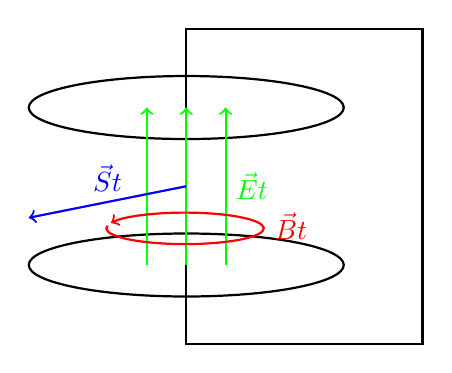
\begin{tikzpicture}
    \coordinate (top) at (0,1);
    \coordinate (bot) at (0,-1);
    \draw[thick] (top) ellipse (2 and 0.4);
    \draw[thick] (bot) ellipse (2 and 0.4);
    \draw[thick] (top) -- (0, 2) -- (3, 2) -- (3, -2) -- (0, -2) -- (bot);
    \draw[thick, green] (top) edge[<-] (bot);
    \draw[thick, green] (0.5, 1) edge[<-] node[midway, right]{$\vec{E}\br{t}$} (0.5, -1);
    \draw[thick, green] (-0.5, 1) edge[<-] (-0.5, -1);
    \draw[thick, blue] (0, 0) edge[->] node[midway, above]{$\vec{S}\br{t}$} (-2, -0.4);
    \draw[->, thick, red] (-1,-0.5) arc [start angle=-190, end angle=160, x radius=1, y radius=0.2];
    \draw[red] (1, -0.5) node[right]{$\vec{B}\br{t}$};
\end{tikzpicture}
\end{center}
We have that the magnetic field points in the $\hat{\phi}$ direction, $\vec{B} = V \hat{\phi}$. The electric field $\vec{E} = E \hat{\zeta}$, and Poynting vector are $\vec{S} = S \hat{s}$. We have that the radiation through the surface $\s{S}$,
\[ \int_{\s{S}} \dif \vec{a} \cdot \vec{S} = - \br{2 \pi a h} S \]
Therefore $\pder{U}{t} = - \br{2 \pi a h} S$ corresponding to the amount of energy flowing out of the capacitor and therefore,
\[ U = \intl_{0}^{\inf} \dif t \br{- 2 \pi a h S} = \f12 C V^2 \]

\textbf{Ex 8.1}:
\begin{center}
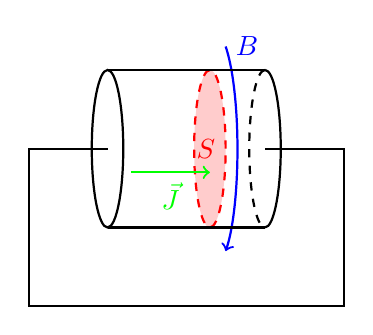
\begin{tikzpicture}
    \pgfmathsetmacro\R{1} % Radius of cylinder
    \coordinate (top) at (\R,0);
    \coordinate (bot) at (-\R,0);
    \coordinate (topshift) at (\R,\R);
    % \draw[thick] (top) ellipse (0.2 and 1);
    \draw[thick] (bot) ellipse (0.2 and 1);
    \draw[thick, dashed] (\R, \R) arc [start angle=90, end angle=270, x radius=0.2, y radius=1];
    \draw[thick] (\R, -\R) arc [start angle=-90, end angle=90, x radius=0.2, y radius=1];
    \draw[thick, blue, <-] (0.5, -1.3) arc [start angle=-60, end angle=60, x radius=0.3, y radius=1.5];
    \draw[thick, blue] (0.5, 1.3) node[right]{$\ve{B}$};
    \draw[thick, dashed, red, fill, fill opacity=0.2] (0.5, 0) arc [start angle=0, end angle=360, x radius=0.2, y radius=1] node[left, fill opacity=1.0]{$\s{S}$};
    \draw[thick] (\R, \R) -- (-\R, \R);
    \draw[thick] (\R, -\R) -- (-\R, -\R);
    \draw[thick] (top) -- (2, 0) -- (2, -2) -- (-2, -2) -- (-2, 0) -- (bot);

    \draw[thick, green] (-0.7, -0.3) edge[->] node[below]{$\vec{J}$} (0.3, -0.3);
\end{tikzpicture}
\end{center}
Inside the conductor the electric field moves parallel to its axis $\vec{E} = \f{V_0}{\ell} \hat{\zeta}$. The magnetic field is then given by,
\[ \vdel \times \vec{B} = \mu_0 \ep_0 \pder{E}{t} + \mu_0 \vec{J} \]
Integration over the surface $\s{S}$,
\[ \int_{\s{S}} \dif \vec{a} \cdot \br{\vdel \times \vec{B}} = \mu_0 \int_{\s{S}} \dif \vec{a} \cdot \vec{J} = \mu_0 I\tsb{enc} \]
Therefore computing this integral $\int \dif \vec{\ell} \cdot \vec{B}$ yields,
\[ \vec{B} = \f{\mu_0I}{2\pi a}\hat{\phi} \]
Moreover, the Poynting vector is given by,
\begin{align*}
\vec{S} &= \f{1}{\mu_0} \vec{E}\times \vec{B} \\
&= \f{1}{\mu_0} \f{V_0}{\ell} \hat{\zeta} \times \f{\mu_0 I}{2 \pi a} \hat{\phi} \\
&= -\f{V_0 I}{2\pi a \ell}\hat{s}
\end{align*}
Therefore the radiation flux,
\[ \int_{\s{S}} \dif \vec{a} \cdot \vec{S} = -\f{V_0 I}{2 \pi a \ell} \int_{\s{S}} \dif a = - V_0 I \]
Which is exactly the amount of Joule heating for a current $I$ though a wire with voltage $V_0$ across it. Using $V = I R$,
\[ \int_{\s{S}} \dif \vec{a} \cdot \vec{S} = -I^2 R \]
\textbf{Ex 8.2 (Griffiths Problem 8.13):}
A long thin solenoid of radius $a$ has a time dependent current $I_{s}\br{t}$ flowing around it. Encircling the solenoid is a ring of radius $b$ with current $I_{r}\br{t}$ ($b \gg a$) passing through it. The ring has resistance $R$. There is an induced electro-motive-force in the ring due to the solenoid,
\[ \s{E} = - \dot{\Phi}_S = - \pder{}{t}\br{\pi a^2 B_S} \]
Where $B_s = \mu_0 n I_s$. The EMF $\s{E}$ must also equal $\s{E} = I_r R$. Therefore,
\[ I_r = - \f{1}{R}\br{\mu_0 \pi a^2 n}\dot{I}_S \]
In order to calculate the electric and magnetic fields just outside solenoid, recognize that $\ve B_s = B_s\br{t} \hat{z}$ point along the axis of the solenoid. Similarly recognize that $\ve E = E \hat{\phi}$. Therefore the Poynting vector is given by,
\[ \ve S = \f{1}{\mu_0} \ve E \times \ve B_s = \f{1}{\mu_0} E B_{s} \hat{s} = ? \]
We first need to calculate $\ve E$ and $\ve B_s$. The magnetic field is known to be $\ve B = \mu_0 n I_s \hat{z}$ on axis and $\vdel \times \ve E = - \pder{\ve B}{t}$,
\[ \int \dif \ve a \cdot \vdel \times \ve E = - \der{}{t} \int \dif \ve a \cdot \ve B \]
\[ \int \dif \ve \ell \cdot \ve E = - \dot \Phi = 2 \pi a E \]
Which gives,
\[ \ve E = \f{\dot \Phi}{2\pi a}\hat{\phi} \]
The magnetic field off axis and outside the solenoid due to the ring is given by,
\[ \dif \ve B_r \br{s} = \f{\mu_0 I}{4 \pi} \f{\dif \ve \ell \times \ve \rcurs}{\rcurs^2} \]
Where $\ve \rcurs = \ve r - \ve r'$ and we take $\ve r ' = b \hat s '$ and $\ve r = z \hat z$.
\[ \ve \rcurs = z \hat z - b \hat s' \]
We will take the infinitesimal loop to be $\dif \ve \ell = b\dif \phi'\hat \phi'$.
\begin{align*}
\dif \ve \ell \times \ve \rcurs &= \br{b \hat \phi' \dif \hat \phi'}\times\br{z\hat z - b \hat s '} \\
&= a z \dif \phi' \hat s' + b^2 \dif \phi' \hat z
\end{align*}
We integrating around the loop $\s{L}$, all of the contributions in the $\hat{s}'$ directions will cancel out.
\[ \int_{\s{L}} \dif \ve \ell \times \ve \rcurs = \cdots \]
Thus,
\begin{align*}
\ve B_r &= \f{\mu_0 I_r}{4\pi} \int \f{b^2 \dif \phi' \hat z}{\br{z^2 + b^2}^{3/2}} \\
&= \f{\mu_0 I_r b^2 2 \pi \hat z}{4\pi \br{z^2 + b^2}^{3/2}} \\
&= \f{\mu_0 b^2}{2\br{z^2 + b^2}^{3/2}}I_r\hat z
\end{align*}
Therefore the Poynting vector points radial outward,
\begin{align*}
\ve S &= \f{1}{\mu_0}\ve E_r \times \ve B_r \\
&= \f{1}{\mu_0}\br{\f{\pi a^2 \mu_0 n \dot I_s}{2 \pi a} \hat \phi} \times \br{\f{\mu_0 b^2}{2\br{z^2 + b^2}^{3/2}}I_r\hat z} \\
&= \f{\mu_0}{4} a n \dot I_s \f{b^2}{\br{z^2 + b^2}^{3/2}} I_r \hat{s}
\end{align*}
Now that the Poynting vector is known, one can calculate the power radiated from the system.
\begin{align*}
P &= \int \dif \ve a \cdot \ve S \\
&= \f{\mu_0}{4} a n \dot I_s I_r b^2 \int \dif z a \dif \phi \hat s \cdot \f{1}{\br{z^2 + b^2}^{3/2}} \hat{s} \\
&= \f{\mu_0}{4} a n \dot I_s I_r b^2 \br{2 \pi a} \int \dif z \f{1}{\br{z^2 + b^2}^{3/2}} \\
&= \f{\mu_0}{4} a n \dot I_s I_r b^2 \br{2 \pi a} \f{2}{b^2} \note{Integral Table} \\
&= \mu_0 \pi a^2 n \dot I_s I_r
\end{align*}
But we know that $\mu_0 \pi a^2 n \dot I_s = - I_r R$. Therefore $P = - I_r^2 R$ as expected.\\
\textbf{A2.2:}\\
a,b) Answers in Griffiths. \\
c) Consider parallel metal strips with height $h$ and width $w$ where $h \ll w$. A current flows down one plate and up the other. The system will act as a capacitor. The magnetic field outside will be zero and non-negative inside. \\
d) Griffiths 8.1 \\
\textbf{A2.3:}\\
Positive and negative charge build up on the surfaces between the capacitor. Of course, there will be a time varying current $I\br{t}$, electric field $\ve E \br{t}$ and magnetic field $\ve B \br{t}$.
\section{Stress Energy Tensor}

Last week we looked at conservation laws and we found,
\[ \vdel \cdot \ve J + \pder{\rho}{t} = 0 \note{(charge)} \]
and,
\[ \vdel \cdot \ve S + \pder{u}{t} + \ve J \cdot \ve E = 0 \note{(energy)} \]
This week we will continue with momentum and angular momentum and then we will examine the Maxwell stress tensor; the field equivalent for force in Newton's second law. But first we will look at momentum.
\subsection{Momentum}
Consider two charges $+q_1$ and $-q_2$ with velocities $\ve v_1$ and $\ve v_2$. The electric field at point $2$ due to charge $1$ will be denoted $\ve E_1$. Analogously for $\ve B_1$. The net force acting on charge $q_2$ is then,
\[ \ve F_{2;E} = q_2 \ve E_1 \qquad \ve F_{2;B} = q_2 \ve v_2 \times \ve B_1 \]
\[ \ve F_{1;E} = q_1 \ve E_2 \qquad \ve F_{1;B} = q_1 \ve v_1 \times \ve B_2 \]
One will notice that $\ve F_{1;B}$ and $\ve F_{2;B}$ are not equal and opposite forces like $\ve F_{1;E}$ and $\ve F_{2;E}$ are. What does this say about Newton's third law?
\[ \sum \dve p_i = \sum \ve F\tsb{net} \]
We forgot about the fact that the electric and magnetic fields carry not only energy (via $\ve S$) but momentum as well. Recall that for photons,
\[ E = h f = \hbar \w  \]
\[ p = \f{h}{\la} = \hbar k \]
Therefore we have that,
\[ E = pc \]
Therefore knowing the energy density of the field gives you then momentum density of the field. The momentum density will be denoted $\ve g$.
\[ \ve g = \f{1}{c^2} \ve S = \mu_0 \ep_0 \ve S = \f{1}{4 \pi c} \ve E \times \ve B \]
Let $\ve f = \De \ve F / \De \tau$ be the force per \textit{unit volume} acting on a particle. The Lorentz force determines the $\ve f$.
\[ \ve f = \rho \ve E + \ve J \times \ve B\]
We can eliminate the dependence on the source terms $\rho$ and $\ve J$ by invoking Maxwell's equations,
\[ \ve f = \ep_0 \br{\vdel \cdot \ve E} \ve E + \br{\f{1}{\mu_0} \vdel \times \ve B - \ep_0 \pder{\ve E}{t}} \times \ve B \]
By product rule,
\[ \pder{}{t}\br{\ve E \times \ve B} = \ve E \times \pder{\ve B}{t} + \pder{\ve E}{t} \times \ve B \]
Invoke Maxwell's equation again $\vdel \times \ve E = - \pder{\ve B}{t}$,
\[ \pder{}{t}\br{\ve E \times \ve B} = -\ve E \times \br{\vdel \times \ve E} + \pder{\ve E}{t} \times \ve B \]
Therefore,
\begin{align*}
\ve f
&= \ep_0 \br{\vdel \cdot \ve E} \ve E + \f{1}{\mu_0} \br{\vdel \times \ve B} \times \ve B - \ep_0 \pder{\ve E}{t}\times\ve B  \\
&= \ep_0 \br{\vdel \cdot \ve E} \ve E + \f{1}{\mu_0} \br{\vdel \times \ve B} \times \ve B - \ep_0 \pder{}{t}\br{\ve E \times \ve B} - \ep_0\ve E \times \br{\vdel \times \ve E}
\end{align*}
Recognize the Poynting vector $\mu_0 \ve S = \ve E \times \ve B$. We will also make use of the product rule for the gradient,
\[ \vdel E^2 = 2 \br{\ve E \cdot \vdel} \ve E + 2 \ve E \times \br{\vdel \times \ve E} \]
After some algebra we arrive at,
\[ \ve f = \ep_0 \bs{\br{\vdel \cdot \ve E} \ve E + \br{\ve E \cdot \vdel} \ve E} + \f{1}{\mu_0} \bs{\br{\vdel \cdot \ve B} \ve B + \br{\ve B \cdot \vdel} \ve B} - \vdel \br{\f{\ep_0}{2} E^2 + \f{1}{2 \mu_0} B^2} - \mu_0 \ep_0 \pder{\ve S}{t} \eq \label{eq:messy}\]
We now introduce \term{Maxwell's stress-energy tensor} $T$ with components,
\[ T_{ij} = \ep_0 \br{E_i E_j - \f{1}{2} \de_{ij} E^2} + \f{1}{\mu_0} \br{B_i B_j - \f{1}{2} \de_{ij} B^2} \eq \label{eq:components_of_MST}\]
Where $\ve E = \sum_{i} E_i \hat{e}_i$ and $\ve B = \sum_{i} B_i \hat{e}_i$. We now have that \cref{eq:messy} gives,
\[ \ve f = \vdel \cdot T - \ep_0 \mu_0 \pder{\ve S}{t} \]
Where the divergence of $T$ can be written as,
\[ \pder{T_{ij}}{x_i} = \ep_0 \br{\pder{E_i}{x_i} E_j + E_i \pder{E_j}{x_i} - \f12 \pder{E^2}{x_j}} + \f{1}{\mu_0} \br{\pder{B_i}{x_i} B_j + B_i \pder{B_j}{x_i} - \f12 \pder{B^2}{x_j}} \]
As defined $\ve F = \int_{\s{V}} \dif \tau \ve f$ is the net mechanical force acting on the matter in a volume $\s{V}$. Therefore,
\begin{align*}
\der{}{t} \ve p\tsb{mech} &= \int_{\s{V}} \dif \tau \ve f \\
&= \int_{\s{V}} \dif \tau \br{\vdel \cdot T - \ep_0 \mu_0 \pder{S}{t}} \\
&= \oint_{\s{S}} \dif \ve a \cdot T - \der{}{t} \int_{\s{V}} \dif \tau \ep_0 \mu_0 \ve S
\end{align*}
We usually define the second term here to be the momentum contained in the electromagnetic field,
\[ \ve p\tsb{em} = \int_{\s{V}} \dif \tau \ep_0 \mu_0 \ve S \]
Therefore the conservation of momentum is,
\[ \der{}{t} \br{\ve p\tsb{mech} + \ve p\tsb{em}} = \oint_{\s{S}} \dif \ve a \cdot T \eq \label{eq:conservation_momentum}\]

To draw intuition from continuum mechanics, the \term{Cauchy stress tensor} is a representation of the total forces acting on a chunk $\s{V}$ of a material due to the neighboring pieces $\s{N}\br{\s{V}}$. Each neighboring chunk $n \br{\s{V}}$ can exert parallel or shear forces on $\s{V}$. This defines a matrix on force components on each face of $\s{V}$. Let $\ve f = \si \cdot \dif \ve a$ where $\ve{\si}$ is a rank 2 (3D) tensor. We call $\si$ the Cauchy stress tensor such that,
\[ \ve f = \si \cdot \dif \ve a \]
The divergence of the Maxwell stress tensor is,
\[ \pder{}{x_i} T_{ij} = \ep_0 \br{\pder{E_i}{x_i}E_j + E_i \pder{E_j}{x_i} - \f12 \de_{ij} \pder{E^2}{x_i}} + \f{1}{\mu_0} \br{\pder{B_i}{x_i}B_j + B_i \pder{B_j}{x_i} - \f12 \de_{ij} \pder{B^2}{x_i}} \]
The divergence can also be written in vector notation.
\[ \vdel \cdot T = \ep_0 \bs{\br{\vdel \cdot \ve E} \ve E + \br{\ve E \cdot \vdel} \ve E} - \f12 \ep_0 \vdel E^2 + \f{1}{\mu_0} \br{\br{\vdel \cdot \ve B} \ve B + \br{\ve B \cdot \vdel} \ve B} - \f12 \ep_0 \vdel B^2 \]
We have just derived that the force per unit volume $\ve f$ satisfies the following equation,
\[ \ve f = \vdel \cdot T - \ep_0 \mu_0 \pder{\ve S}{t} \]
Which can be integrated over a volume $\s{V}$ in order to obtain the total force,
\begin{align*}
\int_{\s{V}} \dif \tau \ve f &= \int_{\s{V}} \dif \tau \vdel \cdot T \\
&= \int_{\s{V}} \dif \tau \vdel \cdot T - \mu_0 \ep_0 \der{}{t} \int_{\s{V}} \dif \tau \ve S\\
\der{\ve p\tsb{mech}}{t}&= \oint_{\s{S}} \dif \ve a \cdot T - \der{}{t} \underbrace{\int_{\s{V}} \dif \tau \ve g}_{\ve p\tsb{em}}
\end{align*}
Therefore we recover \cref{eq:conservation_momentum} again,
\[ \der{}{t} \br{\ve p\tsb{mech} + \ve p\tsb{em}} = \oint_{\s{S}} \dif \ve a \cdot T \]
This conservation of momentum equation can be interpreted as Newton's second law for E\&M. \\

\textbf{Ex 8.4:} Two point charges a distance $2 \ell$ apart. Due to the rotational symmetry of the problem, we can exploit cylindrical coordinates $\ve r = s\hat{s} + z \hat{z}$ because no physical quantities can depend on $\phi$.\\
\textbf{a)} The electric field in a plane ($\phi = 0$) can be obtained as follows. Let $\ve r'$ be the location of the source $q$ and $\ve r$ be the field location. The origin is between the two identical charges. Let $\ve E_{+}$ be the electric field due to the charge in the $z > 0$ direction.
\[ \ve r'_{\pm} = \pm \ell \hat{z} \]
And on the axis perpendicular to $\hat{z}$,
\[ \ve r = s \hat{s} \]
Therefore,
\[ \ve \rcurs = \ve r - \ve r' = s\hat{s} - \ell \hat z \]
Which gives electric field,
\begin{align*}
\ve E_{\pm} &= \f{q_{\pm} \ve \rcurs_\pm}{4 \pi \ep_0 \rcurs_\pm^3} \\
&= \f{q_{\pm}}{4 \pi \ep_0} \f{s \hs \mp \ell \vz}{\br{ s^2 + \ell^2}^{3/2}}
\end{align*}
Therefore,
\[ \vE_{\bc{z = 0}} = \vE_{+} + \vE_{-} = \f{q_{\pm}}{4 \pi \ep_0} \f{2 s \hs}{\br{ s^2 + \ell^2}^{3/2}} \]
Upon reflection, the direction of $\vE_{\bc{z = 0}}$ could have only been in the $\hat s$ direction by symmetry. \\
\textbf{b)} Calculate the Maxwell Stress Tensor using \cref{eq:components_of_MST}. Notice that $\ve B = \ve 0 $ and $\vE_{\bc{z=0}} = E\br{s} \hat{s}$,
\[ \hat{s} = \hat{x}\cos\phi + \hat{y}\sin\phi \]
So in Cartesian coordinates,
\[ \vE_{\bc{z = 0}} = \f{q_{\pm}}{4 \pi \ep_0} \f{2 \sqrt{x^2 + y^2}\br{\hat{x}\cos\phi + \hat{y}\sin\phi}}{\br{ x^2 + y^2 + \ell^2}^{3/2}} \]
The components of $\ve E$ are then,
\[ E_1 = E_x = \f{q_{\pm}}{4 \pi \ep_0} \f{2 \sqrt{x^2 + y^2}\cos\phi}{\br{ x^2 + y^2 + \ell^2}^{3/2}} \]
\[ E_2 = E_y = \f{q_{\pm}}{4 \pi \ep_0} \f{2 \sqrt{x^2 + y^2}\sin\phi}{\br{ x^2 + y^2 + \ell^2}^{3/2}} \]
\[ E_3 = E_z = 0 \]
For convenience let,
\[ E_0 = \f{q_{\pm}}{4 \pi \ep_0} \f{2 \sqrt{x^2 + y^2}}{\br{ x^2 + y^2 + \ell^2}^{3/2}} \eq \label{eq:E_0}\]
Such that,
\[ E_1 = E_0 \cos \phi \quad E_2 = E_0 \sin \phi\]
And also,
\[ E^2 = E_0^2 \]
Therefore the components of $T$ are determined by \cref{eq:components_of_MST},
\[ T = \ep_0 E_0^2 \begin{pmatrix}
    \cos^2 \phi - \f12 & \sin \phi \cos \phi & 0 \\
    \cos \phi \sin \phi & \sin^2 \phi - \f12 & 0 \\
    0 & 0 & - \f12 \\
\end{pmatrix} \]
Which by trig-identities becomes,
\[ T = \f12\ep_0 E_0^2 \begin{pmatrix}
    \cos\br{2\phi} & \sin \br{2\phi} & 0 \\
    \sin \br{2\phi} & -\cos\br{2\phi} & 0 \\
    0 & 0 & - 1 \\
\end{pmatrix} \]
\textbf{c)} Construct a closed hemisphere $\s H$ above $z > 0$ enclosing the charge $q_{+}$ but not $q_{-}$. Since the charges are not moving, we have that,
\[ \der{}{t} \br{\ve p\tsb{mech} + \ve p\tsb{em}} = \ve 0 \]
Therefore it must be,
\[ \oint_{\s{H}} \dif \ve a \cdot T = 0 \]
However, $\s{S}$ does \textit{not} lie in the same plane as the Maxwell stress tensor computed above. Instead, we can take the radius $R$ of the hemisphere to be $R \to \inf$ such that the ``hemisphere'' becomes a flat plane with a central circular region. The net force acting on $q_{+}$ is,
\[ \ve F_{+} = \int_{\s{V}} \dif \tau \ve f = \int_{\s{V}} \dif \ve a  \vdel \cdot T - \ep_0 \mu_0 \der{}{t} \int_{\s{V}} \dif \tau \cancelto{0}{\ve S} = \int_{\s{S}} \dif \ve a \cdot T \]
Therefore,
\begin{align*}
    \ve F_{+} &= \intl_{-\inf}^{\inf} \dif x \intl_{-\inf}^{\inf} \dif y \f12\ep_0 E_0^2 \begin{pmatrix}
        0 & 0 & -1
    \end{pmatrix} \begin{pmatrix}
        \cos\br{2\phi} & \sin \br{2\phi} & 0 \\
        \sin \br{2\phi} & -\cos\br{2\phi} & 0 \\
        0 & 0 & - 1 \\
    \end{pmatrix}\\
    &= \intl_{-\inf}^{\inf} \dif x \intl_{-\inf}^{\inf} \dif y \f12\ep_0 E_0^2 \begin{pmatrix}
        0 \\ 0 \\ 1
    \end{pmatrix}
\end{align*}
Where $E_0 = E_0\br{x,y}$ is given by \cref{eq:E_0}.
\begin{align*}
\ve F_{+} &= \f{1}{2} \ep_0 \hat z \intl_{-\inf}^{\inf} \dif x \intl_{-\inf}^{\inf} \dif y E_0^2 \\
&= \f{1}{2} 2 \pi \ep_0 \br{\f{q}{2 \pi \ep_0}}^2 \hat z \intl_{0}^{\inf} \dif s \f{s \br{s^2}}{\br{s^2+ \ell^2}^{3}} \\
&= \cdots \\
&= \f{q^2 \hat z}{4 \pi \ep_0 \br{2 \ell}^2}
\end{align*}
Which is simply a result of Coulomb's law which was expected.

\subsection{Method of Images}

\textbf{8.4:}
\[ \ve F = \int_{\s{S}} \dif \ve a \cdot T \]
\textbf{A3.1:}
\[ \ve E\tsb{vac} \cdot \hat t = 0 \]
\[ \int \dif \ve \ell \cdot \ve E = 0 \]
\[ \int \dif \ve a \cdot \vdel \times \ve E = - \der{}{t} \int \dif \ve a \cdot \ve B = 0 \]
\[ V\br{x,y,z>0} = V\br{z,y,z} \quad V\br{x,y,z < 0} = 0\]
The boundary condition,
\[ \ve E \cdot \hat n = \f{\si}{\ep_0} \]
Gives the potential at $z = 0^{+}$. \\
Recall that the energy stored in the electromagnetic field is given by,
\[ W = \f{\ep_0}{2} \int \dif \tau E^2 \]
\textbf{A3.?:} The electromagnetic momentum,
\[ \ve g = \mu_0 \ep_0 \ve S = \ep_0 \br{\ve E \times \ve B} \]
The electric field is in the $z$ direction $\ve E = E \hat z$ and the magnetic field is $\ve B = B \hat \phi$. Therefore $\ve S = - S \hat s$. Now consider a charge $q$ and a magnetic dipole $\ve m$ near each other. The magnetic field generated by $\ve m$ and the electric field generated by $q$ generate a joint $\ve S$ field. The $\ve S$ forms closed circles around the system, meaning no energy is moving in or out of the system. Because of this, $\ve g$ is non-zero and is rotational around the system indicating that there is angular momentum stored in the field. The angular momentum density is then,
\[ \ve \ell = \ve r \times \ve g \]
The angular momentum comes from \textit{resisting} the magnetic force in a radial direction when trying to bring the charge $q$ toward the dipole $\ve m$.

\textbf{Feynman Vol. 2 17-4:} Consider a plastic disk that is free to rotate and with surface charge $\si$ (generating field $\ve E$). Then place a solenoid in the center of the disk and turn it on, generating a magnetic field $\ve B$. This field induces an electric field $\ve E'$ in the disk because of Maxwell's law,
\[ \vdel \times \ve E = - \pder{\ve B}{t} \]
Generating some torque $\ve N$, the total angular momentum in the disk is given by,
\[ \ve L\tsb{mech} = \int_{0}^{t} \dif t' \ve N \]
Turning the solenoid on and off transfers angular momentum from the mechanical system to the field system.\\
\textbf{A3.3: (Griffiths 8.4, 8.21):} Solenoid with radius $R$.

\section{Waves}

As it turns out, Maxwell's equations in a vacuum reduce to a pair of similar wave equations. We begin with Maxwell's equations in free space,
\begin{align*}
    \vdel \cdot \ve E &= 0 \\
    \vdel \times \ve E &= -\pder{\ve B}{t} \\
    \vdel \times \ve B &= 0 \\
    \vdel \times \ve B &= \mu_0 \ep_0 \pder{\ve E}{t}
\end{align*}

It is possible to solve these equations by exploiting some vector identities. For an arbitrary vector field $\ve A$,
\[  \vdel \times \br{\vdel \times \ve A} = \vdel \br{\vdel \cdot \ve A} - \vdel^2 A \]
Then take the curl of Faraday's law,
\[ \vdel \times \br{\vdel \times \ve E} = \vdel \times \br{-\pder{\ve B}{t}} \]
Therefore $\vdel \times \br{\vdel \times \ve E} = \vdel \br{\vdel \cdot \ve E} - \vdel^2 E = - \vdel^2 E$,
\[  - \del^2 \ve E = \vdel \times \br{-\pder{\ve B}{t}} \]
But Ampere's law tells us $\vdel \times \ve B$. Therefore,
\[  - \del^2 \ve E = \mu_0 \ep_0 \pdder{\ve E}{t} \]
But we know that $c^2 = 1/\mu_0 \ep_0$ is the speed of the wave. We have derived electromagnetic waves from Maxwell's equations in a vacuum,
\begin{align*}
\del^2 \ve E - \f{1}{c^2} \pdder{\ve E}{t} &= 0 \\
\del^2 \ve B - \f{1}{c^2} \pdder{\ve B}{t} &= 0
\end{align*}
Which is in practice a system of $6$ equations one for each component $f = \bc{E_x, E_y, E_z, B_x, B_y, B_z}$. Today, we will start by examining the 1D wave equation,
\[ v^2 \pdder{f}{z} - \pdder{f}{t} = 0 \eq \label{eq:1d_Wave}\]
Where $v$ is the wave speed and $f\br{z,t}$ is the \textit{displacement} of the \textit{medium} from its equilibrium position. To solve this second order PDE, D'Alembert came up with the substitution,
\[ q_{\pm} = z \pm v t \]
Which has the inversion,
\begin{align*}
\eq \label{eq:dalembert_inversion}
\begin{split}
z &= \f{1}{2}\br{q_{+} + q_{-}} \\
v &= \f{1}{2v}\br{q_{+} - q_{-}}
\end{split}
\end{align*}
This substitution has the following chain rule,
\begin{align*}
    \pder{}{z} &= \pder{q_{+}}{z}\pder{}{q_{+}} + \pder{q_{-}}{z}\pder{}{q_{-}}\\
    \pder{}{t} &= \pder{q_{+}}{t}\pder{}{q_{+}} + \pder{q_{-}}{t}\pder{}{q_{-}}
\end{align*}
So that \cref{eq:1d_Wave} becomes,
\begin{align*}
\pdder{f}{z}
&= \br{\pder{}{q_{+}} + \pder{}{q_{-}}}^2 f \\
&= \pdder{f}{q_{+}} + \pdder{f}{q_{-}} + 2 \f{\di^2 f}{\di q_{+} \di q_-}
\end{align*}
Similarly,
\[ \pdder{f}{t} = v^2\br{\pdder{f}{q_{+}} + \pdder{f}{q_{-}} - 2 \f{\di^2 f}{\di q_{+} \di q_-}} \]
Therefore \cref{eq:1d_Wave} becomes,
\[ \f{\di^2 f}{\di q_{+} \di q_-} = 0 \]
Which has the general solution of a separable function,
\[ f\br{q_+, q_-}= f_+\br{q_+} + f_-\br{q_-} \]
Or in terms of \cref{eq:dalembert_inversion},
\[ f\br{z, t}= f_+\br{z+vt} + f_-\br{z-vt} \]
We will usually write this as:
\[ f\br{z, t}= f_+\br{kz+\w t} + f_-\br{kz-\w t} \eq \label{eq:dalembert_solution} \]
Where $v = \w /k$ and $\w$ is the temporal frequency and $k$ is the spatial frequency. We shall see that the 3D generalization is easy to digest,
\[ f_{\pm}\br{k_z z + k_y y + k_x x \pm \w t} = f_{\pm}\br{\ve k \cdot \ve r \pm \w t} \]
What we will see is that the \term{wave vector} $\ve k$ points in the same direction as the Poynting vector $\ve S$. \\

Due to the linearity of the wave equations, $v^2 \pdder{}{z} - \pdder{}{t}$ can be treated as linear operator $\hat L$ such that,
\[ \hat L \br{\al f + \be g} = \al \hat L \br{f} + \be \hat L \br{g} \]
We can make use of Fourier and his friends so that we only have to solve the wave equation for one frequency (both spatial and temporal). Promote $f\br{z,t}$ to be a complex amplitude $\ti f\br{z, t}$ and then decompose it using spectral analysis,
\[ \ti f\br{z,t} = \int_{-\inf}^{\inf} \dif k e^{i \br{kz - \w t}} f_{k} \br{t} = \s{F}\bs{ \ti f_{k} \br{t}}\br{z,t} \eq \label{eq:fourier}\]
Where $\ti f_{k} \br{t}$ is a complex function of $k$ and $t$ which can be found using an inverse Fourier transform,
\[ \ti f_{k} \br{t} = \f{1}{2\pi}\int_{-\inf}^{\inf} \dif z e^{-i \br{k z - \w t} }\ti f\br{z,t}  \]
To verify that this works, substitute in $\ti f\br{z,t}$ using \cref{eq:fourier},
\begin{align*}
    \f{1}{2\pi} \int_{-\inf}^{\inf} \dif z e^{-i \br{k z - \w t} }\ti f\br{z,t}
    &= \f{1}{2\pi}\int_{-\inf}^{\inf} \dif z e^{-i \br{k z - \w t} }\int_{-\inf}^{\inf} \dif k' e^{i \br{k'z - \w t}} \ti f_{k'} \br{t}f_{k'} \br{t} \\
    &= \f{1}{2\pi}\int_{-\inf}^{\inf} \dif k'  \ti f_{k'} \br{t}f_{k'} \br{t} \int_{-\inf}^{\inf} \dif z e^{-i \br{k z - \w t} } e^{i \br{k'z - \w t}} \\
    &= \f{1}{2\pi}\int_{-\inf}^{\inf} \dif k'  \ti f_{k'} \br{t}f_{k'} \br{t} \int_{-\inf}^{\inf} \dif z e^{-i\br{k - k'} z} \\
    &= 2 \pi \br{\f{1}{2\pi}} \int_{-\inf}^{\inf} \dif k'  \ti f_{k'} \br{t}f_{k'} \br{t} \de\br{k - k'} \\
    &= \ti f_{k} \br{t}
\end{align*}
We write as shorthand,
\[ \ti f_k \br{t} = \s{F}^{-1}\bs{\ti f\br{z,t}}_k \br{t} \]
Recovering the actual solution to the wave equation corresponds to taking the real part to $\ti f$,
\[ \Re \bs{\ti f \br{z, t}} = \Re \bs{\abs{\ti f}e^{i \de}} = \abs{\ti f}\cos\br{\de} \]

\textbf{Ex. 9.1:}
\textbf{a)}
\[ \cos \br{A + B} = \cos \br{A} \cos \br{B} - \sin \br{A} \sin \br{B} \]
Therefore,
\[ y_1\br{x,t} = A_1 \cos\br{kx - \w t} \cos S_1 - A_1 \sin\br{kx - \w t} \sin S_1 \]
\[ y_2\br{x,t} = A_2 \cos\br{kx - \w t} \cos S_2 - A_2 \sin\br{kx - \w t} \sin S_2 \]
Combining yields, \\
\textbf{b)}
\[ y\br{x,t} = \underbrace{\br{A_1 \cos S_1 + A_2 \cos S_2}}_{a}\cos\br{k x - \w t} - \underbrace{\br{A_1 \sin S_1 + A_2 \sin S_2}}_{b}\sin\br{k x - \w t} \]
\textbf{c)}
\[ y\br{x,t} = \sqrt{a^2 + b^2} \br{\f{a}{\sqrt{a^2 + b^2}} \cos \br{kx - \w t} - \f{b}{\sqrt{a^2 + b^2}} \sin \br{kx - \w t}} \]
\textbf{d)}
\[ y\br{x,t} = A \cos \br{kx - \w t + \de} \]
Where,
\[ A = \sqrt{a^2 + b^2} \quad \de = \tan^{-1}\br{\f{b}{a}} \]
\textbf{e)}
\[ y\br{x,t} = \sqrt{A_1^2 + A_2^2 + 2 A_1 A_2 \cos \br{\de_1 - \de_2}}\sin\br{kx - \w t + \tan^{-1}\br{\f{A_1 \sin \de_1 + A_2 \sin \de_2}{A_1 \cos \de_1 + A_2 \cos \de_2}}} \]
\textbf{f)}
\[ y_1 = \Re \bc{A_1 e^{i \de_1} e^{i \br{kx - \w t}}} \]
\[ y_2 = \Re \bc{A_2 e^{i \de_2} e^{i \br{kx - \w t}}} \]
Abusing notation a little bit,
\[ y = y_1 + y_2 = \Re\bc{\br{A_1 e^{i\de_1} + A_2 e^{i\de_2}} e^{i \br{kx - \w t}}} \]
\begin{align*}
A^2
&= \br{A_1 e^{i \de_1} + A_2 e^{i \de_2}}\br{A_1 e^{-i \de_1} + A_2 e^{-i \de_2}} \\
&= \cdots \\
&= A_1^2 + A_2^2 + 2 A_1A_2 \cos \br{\de_1 - \de_2}
\end{align*}
\begin{align*}
\tan \de
&= \f{\Im\bc{A_1 e^{i \de_1} + A_2 e^{i \de_2}}}{\Re\bc{A_1 e^{i \de_1} + A_2 e^{i \de_2}}} \\
&= \cdots \\
&= \f{A_1 \sin \de_1 + A_2 \sin \de_2}{A_1 \cos \de_1 + A_2 \cos \de_2}
\end{align*}

\textbf{Ex. 9.2:}
\begin{center}
    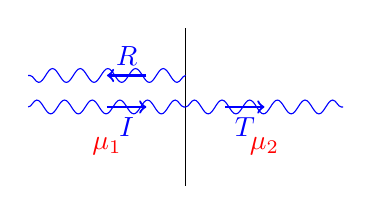
\begin{tikzpicture}
        \draw (0, -1) -- (0, 1);
        \draw [blue,decorate, decoration=snake] (-2, 0) -- (0,0);
        \draw [blue,decorate, decoration=snake] (0, 0.4) -- (-2,0.4);
        \draw [blue,decorate, decoration=snake] (0, 0) -- (2,0);
        \draw [blue, ->, thick] (-1, 0) -- node[below]{$I$} (-0.5,0);
        \draw [blue, ->, thick] (0.5, 0) -- node[below]{$T$} (1,0);
        \draw [blue, ->, thick] (-0.5, 0.4) -- node[above]{$R$} (-1,0.4);
        \draw [red] (-1, -0.5) node[]{$\mu_1$};
        \draw [red] (1, -0.5) node[]{$\mu_2$};
    \end{tikzpicture}
\end{center}

\[ y_I\br{x,t} = A_I \sin \br{k_1 \br{x - v_1 t}} \]
\[ y_R\br{x,t} = A_R \sin \br{k_1 \br{x + v_1 t}} \]
\[ y_T\br{x,t} = A_T \sin \br{k_2 \br{x - v_2 t}} \]
\textbf{a)}
\[ \w_1 = \w_2 \implies k_1 v_1 = k_2 v_2 \]
This means that the ``knot'' at the interface is a ``good'' knot -- i.e. the string at either side of the interface ($x=0$) move with the same frequency -- i.e. the strings are connected.\\

\textbf{b)}

\begin{center}
    \begin{tikzpicture}
        \draw[fill] (0,0) circle (0.05);
        \draw[thick,->] (0,0) -- (1,1) node[above right]{$\ve F_2$};
        \draw[thick,->] (0,0) -- (-1,-0.6) node[below left]{$\ve F_1$};
    \end{tikzpicture}
\end{center}

\[ m \ve a\tsb{net} = \ve F_1 + \ve F_2 \]
If the slopes are the same then $\ve F_1 \parallel \ve F_2$ and so $\ve a\tsb{net}$ is also parallel.

\begin{center}
    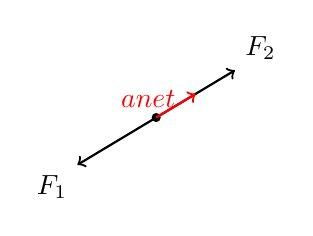
\begin{tikzpicture}
        \draw[fill] (0,0) circle (0.05);
        \draw[red] (-0.1,0) node[above]{$\ve a\tsb{net}$};
        \draw[thick,->] (0,0) -- (1,0.6) node[above right]{$\ve F_2$};
        \draw[thick,->] (0,0) -- (-1,-0.6) node[below left]{$\ve F_1$};
        \draw[thick,red, ->] (0,0) -- (0.5,0.3);
    \end{tikzpicture}
\end{center}
By the principle of superposition the equations for the waves in the first medium can be simply added together,
\[ y_1 \br{x,t} = y_I\br{x,t} + y_R\br{x,t} \]
\[ y_2 \br{x,t} = y_T\br{x,t} \]
Introduce the constraints of a good string,
\[ y_1\br{x=0, t} = y_2\br{x=0, t} \]
Therefore,
\[ A_I \sin\br{-k_1 v_1 t} + A_R \sin\br{k_1 v_1 t} = A_T \sin\br{-k_2 v_2 t} \]
Therefore,
\[ - A_I + A_R = - A_T \]
Equivalently,
\[ A_I = A_R + A_T \]
\textbf{d)}
The next constraint imposes,
\[ \pder{}{x}y_1\br{x=0, t} = \pder{}{x}y_2\br{x=0, t} \]
\[ k_1A_I \cos\br{-k_1 v_1 t} + k_1A_R \cos\br{k_1 v_1 t} = k_2A_T \cos\br{-k_2 v_2 t} \]
Thus,
\[ k_1 A_I + k_2 A_R = k_2 A_T \]
Now solve for the reflected and transmitted $A_R, A_T$ in terms of the given incidence amplitude. So,
\[ A_R = \f{v_1 - v_2}{v_1 + v_2} A_I \]
\[ A_T = \f{2v_2}{v_1 + v_2} A_I \]
\textbf{e)}
If $v_2 > v_1$ then $A_R \propto - \br{A_I}$.

\subsection{Polarization}
So far, we have only considered 1D waves. However, the electric and magnetic fields are vector quantities. As we shall see shortly, EM radiation has field components that are perpendicular to the direction of propagation. We can thus write a traveling wave as
\[ \ti {\ve f}\br{z, t} = \ti f_{k} \hat n e^{i\br{kz - \w t}} \]
Where $e^{i\br{kz - \w t}}$ acts as the traveling wave, $\hat n$ is the polarization and $\ti f_{k}$ is the amplitude and phase. Note that $\ti f_{k}$ is not a function of position $\ve r$ and time $t$. The possible polarizations of this plane wave are $\hat x, \hat y$ or a linear combination thereof. An important linear combination is,
\[ \hat n_{\pm} = \hat x \pm i \hat y = \hat x \pm e^{i \pi / 2} \hat y \]
So that,
\[ \hat n_{\pm} e^{i\br{kz - wt}} = \hat x e^{i\br{kz - wt}} \pm \hat y e^{i\br{kz - wt + \pi/2}}\]
Which makes the total wave,
\begin{align*}
\Re\bc{\ti f_{k}\hat n_{\pm} e^{i\br{kz - wt}}}
&= \Re\bc{\abs{\ti f_{k}} e^{i \de} \hat n_{\pm} e^{i\br{kz - wt}}} \\
&= \abs{\ti f_{k}}\Re\bc{\br{\hat x + i \hat y} \br{\cos \br{kz - wt + \de} + i\sin \br{kz - wt + \de}}} \\
&= \abs{\ti f_{k}}\br{\hat x \cos \br{kz - wt + \de} - \hat y\sin \br{kz - wt + \de}} \\
\end{align*}

\begin{center}
    \begin{tikzpicture}
        \pgfmathsetmacro\rs{1.5}
        \draw (-2, 0) -- (2, 0) node[right]{$x$};
        \draw (0, -2) -- (0, 2) node[above]{$y$};
        \draw[red, ->] (0,0) -- (\rs, 0) node[above right]{$t = 0$};
        \draw[green, ->] (0,0) -- ({cos(60)*\rs}, {sin(60)*\rs}) node[above right]{$t = 2\De t$};
        \draw[green, ->] (0,0) -- ({cos(90)*\rs}, {sin(90)*\rs}) node[above]{$t = 3\De t$};
        \draw[green, ->] (0,0) -- ({cos(30)*\rs}, {sin(30)*\rs}) node[above right]{$t = \De t$};
    \end{tikzpicture}
\end{center}

\subsection{EM Plane Waves}
While this is sufficient for a generic wave equation however, for those satisfying Maxwell's Equations there are further conditions to impose. In particular, for a plane wave traveling in the $z$-direction we have,
\[ \ti {\ve E} \br{z, t} = \ti{\ve E}_0 e^{i\br{k z - \w t}} \]
With derivatives,
\[ \pder{}{x} \ti {\ve E} = \pder{}{y} \ti {\ve E} = \ve 0 \]
\[ \pder{}{z} \ti {\ve E} = ik \ti {\ve E} \]
\[ \pder{}{t} \ti {\ve E} = -i\w \ti {\ve E} \]
We will write,
\[ \ti{{\ve E}}_0 = \hat x \ti {E}_{0, x} + \hat y \ti {E}_{0, y} + \hat z \ti {E}_{0, z} \]
And similarly for the magnetic field,
\[ \ti {\ve B}_0 = \hat x \ti {B}_{0, x} + \hat y \ti {B}_{0, y} + \hat z \ti {B}_{0, z} \]
Note that this is not the same as the electric field itself,
\[ \ti E_x = \ti{\ve E} \cdot \hat x = \ti{\ve E}_0 \cdot \hat x e^{i \br{kz - \w t}} = \ti{E}_{0,x} e^{i \br{kz - \w t}} \]
Next make use of Gauss's law (in vacuum),
\[ 0 = \vdel \cdot \ve E = \ti E_{0,z} i k e^{i\br{kz - \w t}} \implies \ti E_{0,z} = 0 \]
Similarly for $\ve B$,
\[ \ti B_{0,z} = 0 \]
So that EM waves are \textit{transverse} and $\ti {\ve E}_0$ only has components in the $\hat x$ and $\hat y$ directions.\\

Moreover make use of Faraday's law,
\[ \vdel \times \ve E = - \pder{\ve B}{t} \]
Which gives,
\[ - i k \hat x \ti E_y + i k \hat y \ti E_x = i \w \br{ \hat x \ti B_x + \hat y \ti B_y + \hat z \ti B_z} \]
Therefore matching components,
\begin{align*}
    -i k \ti E_y &= i \w \ti B_x \\
    i k \ti E_x &= i \w \ti B_y \\
    0 &= i \w \ti B_z
\end{align*}
Which makes,
\begin{align*}
    \ti E_y &= - \f{\w}{k} \ti B_x = - c \ti B_x \\
    \ti E_x &= + \f{\w}{k} \ti B_y = + c \ti B_y
\end{align*}
And so $\ti{\ve E}$ and $\ti{\ve B}$ have the same phase but are in the different directions. In this case, we can write $c \ti{\ve B} = \hat z \times \ti{\ve E}$ so that the set $\bc{\ti{\ve E} , \ti{\ve B} , \hat z}$ form a right-hand set (which was already known from $\mu_0 \ve S = \ve E \times \ve B$). We can generalize this to a plane wave traveling in an arbitrary direction by introducing the \term{wave vector} $\ve k = k_x \hat x + k_y \hat y + k_z \hat z$. Also,
\[ \ve k = k \hat k = \sqrt{k_x^2 + k_y^2 + k_z^2} \hat k \]
The recurring relation $k z - \w t$ becomes,
\[ \ve k \cdot \ve r - \w t  \]
Monochrome plane waves in vacuum traveling in the $\hat k$ direction are,
\begin{align*}
\ti{\ve E}\br{\ve r , t} &= \ti{\ve E}_0 e^{i\br{\ve k \cdot \ve r - \w t}} \\
c\ti{\ve B}\br{\ve r , t} &= \hat k \times \ti{\ve E}\br{\ve r , t}
\end{align*}
The quantity $\ti{\ve E}_0 = \hat x \ti{E}_{0,x} + \hat y \ti{E}_{0,y} + \hat z \ti{E}_{0,z} = \hat n E_0 e^{i \de}$ represents the polarization, amplitude, and phase of the wave but contains no space or time dependence.
\subsection{Energy and Momentum}
We are now equipped with the general setting of a monochromatic plane wave traveling in a direction $\hat k$. It has already been seen that $\hat k$ is in the same direction as the Poynting vector $\ve S$ which points in the direction of electromagnetic radiation. $\ve S$ satisfies Poynting's theorem,
\[ \vdel \cdot \ve S + \pder{u}{t} + \ve E \cdot \ve J = 0 \]
Which in a vacuum indicates that $\ve S \cdot \dif \ve a$ is the amount of energy flowing out of a point in a time $\dif t$. Therefore the electromagnetic waves previously discussed are carrying electromagnetic energy. The electromagnetic energy density is,
\[ u = \f{\ep_0}{2}E^2 + \f{1}{2 \mu_0} B^2 \]
But for electromagnetic waves, $B^2 = \mu_0 \ep_0 E^2$. Thus
\begin{align*}
    u = \f{\ep_0}{2} E^2 + \f{1}{2\mu_0} \mu_0 \ep_0 E^2 = \ep_0 E^2
\end{align*}
Which for a monochromatic 1D wave becomes,
\[  u = \ep_0 E_0^2 \cos^2\br{kz - \w t + \de} \]
At a point $z$ at time $t$ there is local energy density of $u\br{z,t}$ stored in the electromagnetic field. The Poynting vector however is,
\[ \ve S = \f{1}{\mu_0} \ve E \times \ve B = \f{1}{\mu_0} \ve E \times \br{\f{1}{c} \ve k \times \ve E} \]
Which by a triple product vector identity $\ve A \times \br{\ve B \times \ve C} = \ve B \br{\ve A \cdot \ve C} - \ve C \br{\ve A \cdot \ve B}$ yields,
\[ \ve S = \f{1}{c \mu_0} \bs{\ve k E^2 - \ve E \br{\ve E \cdot \ve k}} \]
But $\ve k$ is orthogonal to $\ve E$,
\[ \ve S = \f{1}{c\mu_0} E^2 \ve k = c\ep_0 E^2 \ve k = c u \ve k \]
This is remarkable. The Poynting vector indicates that there is a flow of energy per unit area per unit time of $c u$ in the $\ve k$ direction.

\subsection{Electromagnetic Waves in Media}

\todo[TC]{Missed a lecture}

In alternative media that are not linear, isotropic, and homogeneous, Maxwell's equations are nearly identical; the only necessary modification is to replace the speed of propagation $c$ with a speed $v$ that is dependent on the material.
\[ c = \f{1}{\sqrt{\ep_0 \mu_0}} \mapsto v = \f{1}{\sqrt{\ep \mu}} \]

In a higher level course, one would explore how to modify Maxwell's equations for materials that do not obey the assumptions of linearity, isotropy, and homogeneity. Doing so is of great importance; material sciences are a very versatile field of physics with countless applications. \\

If one has a dielectric media adjacent to vacuum and a light source emanating isotropically, there are two contributions to light incident on an observer sitting on the interface: the source ray, and the ray reflected off the vacuum dielectric interface.

\begin{center}
    \begin{tikzpicture}
        \draw[] (-3, 0) -- (3,0);
        \draw (3,2) node[](source){$S$};
        \draw (-2,0.5) node[](obs){$O$};
        \coordinate (r) at (-0.2,0);
        \begin{scope}[decoration={markings, mark=at position 0.5 with {\arrow{>}}}]
            \draw[thick, postaction={decorate}] (source) -- node[below right]{$\ve k$} (r);
            \draw[thick, postaction={decorate}] (r) -- (obs);
            \draw[thick, postaction={decorate}] (source) -- (obs);
            \draw[dashed, thick, postaction={decorate}] (r) -- (-1.6, -1);
        \end{scope}
        \draw (2,0) node[above right]{Vacuum};
        \draw (2,0) node[below right]{Dielectric};
        \draw (r) -- (-0.2, 2);
        \draw (-0.2, 0.2) node[above left]{$\te_{R}$};
        \draw (-0.2, 0.2) node[above right]{$\te_{I}$};
    \end{tikzpicture}
\end{center}

The reflected ray is polarized horizontally upon reflecting off the surface of the medium.

\subsection{Conductors}

Inside a conductor we have,
\[ \ve J_f = \si \ve E \eq \label{eq:ohms_law}\]
Where $\si$ is the conductivity, $\ve J_f$ is the free current density and $\ve E$ is the electric field. More generally $\si$ can be a tensor that has components for every pair of directions. However for homogeneous and isotropic media, we can take the conductivity to be a scalar quantity. In contrast, the bound current density $\ve J_b$ is the set of moving charges that are bound to atoms in the material. Specifically the \textit{ensemble} of electrons bound orbitally to atoms contribute a current that flows through the medium (typically surface currents).\\

\Cref{eq:ohms_law} is called \term{Ohm's law}. Ohm's law is typically introduced as $V = IR$. The $V = IR$ equation is a consequence of the local equation that is \cref{eq:ohms_law} together with the assumptions of homogeneity and isotropy. \\

Recall that for constant electric fields, Ohm's law holds initially. However, the electric field with polarize the material to the point where the internal induced electric field exactly cancels the applied electric field. The system approaches equilibrium. \\

However for time depended electric fields, the material's polarization with be a function of time as well. Considering the applied field as an oscillation at frequency $f$, the material's amplitude of oscillation will peak at its resonant frequency. Moreover, there will be a phase shift at the resonant frequency as well.

\subsection{Absorption \& Dispersion}

Inside a conductor we have $\ve J_f = \si \ve E$ where $\si$ is the conductivity (resistivity is $1/\rho$). Maxwell's equations now take the form,
\begin{align*}
    \vdel \cdot \ve E &= \f{1}{\ep} \rho_{f} \\
    \vdel \cdot \ve B &= 0 \\
    \vdel \times \ve E &= -\pder{\ve B}{t} \\
    v^2\vdel \times \ve B &= \pder{\ve E}{t} + \f{1}{\ep} \ve J_f
\end{align*}
We now replace the final term in the last maxwell equation and write,
\[ v^2\vdel \times \ve B = \pder{\ve E}{t} + \f{\si}{\ep} \ve E \]
From this we are able to derive wave equations,
\[ \vdel \times \br{\vdel \times \ve E} = - \pder{}{t}\br{\vdel \times \ve B} \]
\[ \vdel \br{\vdel \cdot \ve E} - \del^2 \ve E = -\f{1}{v^2} \pder{}{t}\br{\pder{\ve E}{t} + \f{\si}{\ep} \ve E} \]
But we have that $\vdel \cdot \ve E = \f{1}{\ep} \rho_{f}$. In a conductor $\rho_{f} \approx 0$ because the time scale to equilibrate $\tau_{d} = \f{\ep}{\si} \approx \SI{1e-20}{\s}$ is short (of course if your frequency is $f \geq \tau_d^{-1}$ this approximation doesn't hold).
Therefore we arrive at,
\[ v^2 \del^2 \ve E = \pdder{\ve E}{t} + \f{\si}{\ep} \pder{\ve E}{t} \]
The ansatz is (for a 1D system) is identical to the dispersion-less case but with $k \to \ti k$,
\[ \ti{\ve E}\br{z,t} = \ti{\ve E}_0 e^{i\br{\ti k z - \w t}} \]
The imaginary component of $\ti k$ introduces an exponential dampening. This leads to an auxiliary equation,
\[ \ti k^2 = \mu \ep \w^2 + i \mu \si \w \]
Which has solution $\ti k = k + i \kappa$ where,
\begin{align*}
    k &= \w \sqrt{\f{\ep \mu}{2}} \sqrt{\sqrt{1 + \br{\f{\si}{\ep \w}}^2}+1} \\
    \kappa &= \w \sqrt{\f{\ep \mu}{2}} \sqrt{\sqrt{1 + \br{\f{\si}{\ep \w}}^2}-1}
\end{align*}
Notice that $\f{\si}{\ep \w}$ is dimensionless. Note that $k \neq \abs{\ti k}$
\todo[TC]{Missed a lecture}

\textbf{A6.1:} \textbf{a)} We have that,
\[ \ve E_I \br{\ve r, t} = \ve E_{I_0} e ^{i \br{\ve k_I \cdot \ve r - \w t}} \]
Where $\ve E_{I_0} = E_0 \hat e_1$ and $\ve k_{\mp} = k \hat e_2$ and the $\hat e_i$ are unit vectors. What are the $\hat e_1$ and $\ve e_2$.

\begin{center}
    \begin{tikzpicture}
        \draw (-3, 0) -- (3, 0);
        \coordinate (o) at (0, 0);
        \coordinate (I) at (-1, 2);
        \coordinate (R) at (1, 2);
        \begin{scope}[decoration={markings, mark=at position 0.5 with {\arrow{>}}}]
            \draw[thick, postaction={decorate}] (I) -- node[left]{$\ve k_I$} (o);
            \draw[thick, postaction={decorate}] (o) -- node[right]{$\ve k_R$} (R);
        \end{scope}
        \draw[->] (I) -- ($(I) + (0.5, 0.25)$) node[above]{$\ve E_I$};
        \draw[->] (R) -- ($(R) + (-0.5, 0.25)$) node[above]{$\ve E_R$};
        \draw[dashed] (o) -- ($(o) + (0, 3)$);
        \draw ($(o) + (-0.2, 1)$) node[]{$\te$};
        \draw (2, 0) node[above]{vacuum};
        \draw (2, 0) node[below]{conductor};
    \end{tikzpicture}
\end{center}

\textbf{b)} For the reflected ray,
\[ \ve E_R \br{\ve r, t} = \ve E_{R_0} e^{i \br{\ve k_R \cdot \ve r - \w t}} \]
where $\ve E_{R_0} = E_0 \hat e_3$ and $\ve k_R = k \hat e_4$. What are the the $\hat e_i$?\\
\textbf{c)} What are the $\ve E$ and $\ve B$ boundary conditions and where do they come from? Make pill boxes on the interface. \\
\textbf{d)} What is $\ve E \mid_{z = 0}$ in terms of $E_0, k, \te, x, y, t$ and $\hat x, \hat y, \hat z$. Hint: we know that it is parallel to the plane of incidence by construction for really there is no need to consider $\hat x, \hat y$ directions. Since $\ve k_R \cdot \ve r = k \hat e_4 \cdot \ve r = kx \hat e_4 \cdot \hat x = kx \sin \te$
\[ \ve E \mid_{z= 0} = 2 E_0 \hat z \sin \te \cos \br{kx\sin\te - \w t} \]
\textbf{e)} What is $\si = ?$ \\
\textbf{f)} Recall that $\ve B = \f{\ve k}{\w} \times \ve E = \f{\hat k}{c} \times \ve E$ and then find $\ve B_I \br{\ve r, t}$? \\
\textbf{g)} The reflected $\ve B_R\br{\ve r, t}$ can be calculated as well. \\
\textbf{h)} What are the $\ve B$ boundary conditions at the inteface? \\
\textbf{i)} What is $\ve B \mid_{z = 0}$? \\
\textbf{j)} We have that $\mu_0 \ve K = \ve B \times \hat n$ which means that $\ve K$ is in the $\hat x$ direction. \\
\textbf{k)} What is the velocity $\ve v$ of the charge at the surface? Does this make sense?

\subsection{Frequency Dependence of Permittivity}
Electromagnetic wave propagation depends on $\ep, \mu$ and $\si$ and we have, so far, assumed that these are frequency independent. If we elevate $\mu, \ep$ and $\si$ to depend on $\w$ we have that,
\[ v\br{\w} = \f{1}{\sqrt{\mu\br{\w} \ep \br{\w}}} \]
This phenomena is know as \term{dispersion}. The index of refraction is modified also,
\[ n \br{\w} = \f{c}{v\br{\w}} \]
Any wave packet will have a \term{phase velocity} (the speed of the surfaces of constant phase),
\[ v = \f{\w}{k} = f \la \]
While the \term{group velocity} is the speed of the wave packet.
\[ v_g = \der{\w}{k} = \f{\dif E / \dif k}{\dif E / \dif \w} \]
We will learn that $v v_g = c^2$ always.\\

In order to get a mathematical model for this, let's look at the 1D, damped, driven, harmonic oscillator.
\[ m \ddot {\ti x} = - m\w_0^2 {\ti x} - m \ga \dot {\ti x} + F_0 e^{i \w t} \]
Where $m \ga \dot {\ti x}$ and $F_0 e^{i \w t}$ is a driven force. This equation motivates the ansatz,
\[ x\br{t} = \Re\br{\ti x_0 e^{i\w t}} \]
Which induces the auxiliary equation,
\[ - \w^2 \ti x_0 - i \ga \w \ti x_0 + \w_0^2 \ti x_0 = \f{F_0}{m} \]
Rearranging,
\[ \ti x_0 = \f{F_0}{m} \f{1}{\w_0^2 - \w^2 - i \ga \w} = \f{F_0}{m} \f{\br{\w_0^2 - \w^2} + i \ga \w}{\br{\w_0^2 - \w^2} + \br{\ga \w}^2} = x_0 e^{i \de} \]
If $\ti{F}\br{t} = w E_0 e^{i \w t}$ then the dipole moment of the oscillator will be the real part of $\ti p \br{t} = \w \ti x \br{t}$ where $\ti p \br{t}$ is,
\[ \ti p \br{t} = \f{q^2 E_0 e^{i \w t}}{m} \f{1}{\w_0^2 - \w^2 - i \ga \w} = \f{q^2 E_0 e^{i \w t}}{m} \f{\br{\w_0^2 - \w^2} + i \ga \w}{\br{\w_0^2 - \w^2} + \br{\ga \w}^2} \]
So that $\ti p \br{t}$ an $\ti E\br{t}$ will have a phase difference,
\[ \de = \tan^{-1} \br{\f{\ga \w}{\w_0^2 - \w^2}} \]
So that the phase difference itself is frequency dependent. \\

We now have the result for a damped, driven, harmonic oscillator and found the  polarization to be,
\[ \ti{p}\br{t} = \f{q^2 E_0 e^{-i\w t}}{\ep_0 m} \f{1}{\w_0^2 - \w^2 - i \ga \w} \]
This result holds for a single oscillator with natural frequency $\w_0$ and damping $\ga$ ($\w$ is the frequency of the driving force and $\w_0$ is the natural frequency).\\

For polarizable media we have many oscillators and we can write the polarization density as,
\[ \ti{\ve P}\br{\w} = \f{N q^2}{\ep_0 m} \bc{\sum_{j} \f{f_j}{\w_j^2 - \w^2 - i \ga_j \w}} \ti{\ve E}\br{\w} \]
Recall that $\ve E = \ve D - \ve P$ and $\ve E = \ep \ve D, \ve P = \ep_0 \chi \ve E$. Where the susceptibility is,
\[ \chi = \f{N q^2}{\ep_0 m} \bc{\sum_{j} \f{f_j}{\w_j^2 - \w^2 - i \ga_j \w}} \]
Previously, this was taken to be a constant but now it is frequency dependent $\chi \mapsto \chi\br{\w}$. It is convenient to introduce the complex dielectric constant,
\[ \ti \ep = \ep_0 \br{1 + \ti \chi} \]
We make the approximation that $\ti \chi$ is reasonably small such that we can make the approximation,
\[ \sqrt{\ti \ep} \approx \sqrt{\ep} \br{1 + \f12 \ti \chi} \]
And the wave equation can be rewritten as,
\[ \del^2 \ti{\ve E} = \ti \ep \mu_0 \pdder{\ti{\ve E}}{t} \]
With solution,
\[ \ti{\ve E}\br{z, t} = \ti{\ve E}_0 e^{i\br{\ti k z - \w t}} = \ti{\ve E}_0 e^{- \Im\br{\ti k} z} e^{i\br{\Re\br{\ti k} z - \w t}} \]
Where,
\[ \ti k = \w \sqrt{\ti \ep \mu_0} = \f{\w \sqrt{\ti \ep \mu_0}}{c \sqrt{\ep \mu_0}} = \f{\w}{c}\br{1 + \f{N q^2}{2 m \ep_0} \sum_j \f{f_j}{\w_j^2 - \w^2 - i \ga_j \w}} \]
And the refractive index is,
\[ n = \f{c}{v} = \f{ck}{\w} = \f{c}{\w} \Re\br{\ti k} \]
\[ n \approx 1 + \f{N q^2}{2 m \ep_0} \sum_j \f{f_j\br{\w_0^2 - \w^2}}{\br{\w_j^2 - \w^2}^2 + \br{\ga_j \w}^2} \]
We make a distinction: \term{Normal Dispersion} occurs when $\dif n / \dif \la > 0$ while \term{Anomalous Dispersion} occurs when $\dif n / \dif \la < 0$. (do not get confused here; $n = \f{c}{v} = \f{c}{\la f} = \f{c k}{\w}$ holds for always)\\
While the absorption coefficient is $\al = 2 \Im\br{\ti k}$,
\[ \al \approx \f{N q^2 \w^2 }{m c \ep_0} \sum_j \f{f_j \ga_j}{\br{\w_j^2 - \w^2}^2 + \br{\ga_j \w}^2} \]
\subsection{Plasma Frequency}
In the high frequency limit we can expand the sum.
\[ \ti k \sqrt{\ti \ep \mu_0} \w = \f{\w}{c} \sqrt{\ti \ep} = \f{\w}{c} \br{1 + \f{N q^2}{m} \sum_j \f{f_j}{\w_j^2 - \w^2 - i \ga_j \w}} \approx \f{\w}{c}\br{1 - \f{NZ q^2}{m \w^2}} \]
Where $Z = \sum_j f_j$ is the number of electrons per unit volume. This can be wrtitten as $\ti n = \f{c \ti k}{\w} = 1 - \f{\w_p^2}{\w^2}$ where,
\[ \w_p^2 = \f{Nq^2 Z}{m} \]
Is the \term{plasma frequency}.

\todo[TC]{Missed 3 lectures}

Last time we were examining TE waves and found that the transvere part, $\ti{\ve E}_{\perp}$, was the same as for the DC system we investigated earlier and the longitudinal part $\hat z \ti{B}_z$, was a traveling wave. The boundary conditions led us to the ansatz,
\[ \ti{\ve E}\br{\ve r, t} = \hat y E_0 \sin\br{k_x x} e^{i\br{k_z z - \w t}} \eq \label{eq:rect_waveguide_ansatz}\]
For a traveling wave in a rectangular waveguide we substitute \cref{eq:rect_waveguide_ansatz} into Maxwell's equations,
\[ \vdel \cdot \ve E = \pder{}{y}E_y = 0 \]
Which is satisfied by \cref{eq:rect_waveguide_ansatz}. Next we would like to check this ansatz against $\vdel \times \ve E = - \pder{\ve B}{t}$ but this can get messy. Instead check the wave equation for $\ve E$,
\[ \del^2 \ti{\ve E} - \mu \ep \pdder{\ti{\ve E}}{t} = 0 \]
In Cartesian coordinates,
\[ \br{\pdder{}{x} + \pdder{}{y} + \pdder{}{z} - \mu \ep \pdder{}{t}}\ti{\ve E} = 0 \]
This leading operator is the \term{D'Alembertian operator}\footnote{Sometimes you will see this written as $\Box$ or $\Box^2$. This is reminiscent of special relativity where $\de_\mu = \br{\mu \ep \pder{}{t}, \vdel}$},
\[ \Box^2 = \pdder{}{x} + \pdder{}{y} + \pdder{}{z} - \mu \ep \pdder{}{t} \]
Applying the wave equation we obtain an auxiliary equation.
\[ \Box^2 \ti{\ve E} = \br{- k_x^2 + 0 - k_y^2 + \mu \ep \w^2} \ti{\ve E} = 0 \]
Avoiding the trivial solution, we require that,
But in order to meet the boundary conditions of the rectangular waveguide,
\[ k_x = \f{m \pi}{a} \quad m \in \N \]
So that $k_z$ is fixed as well,
\[ k_z = \sqrt{\mu \ep \w^2 - \br{\f{m \pi}{a}}^2} \]
\[ k_z = \f{\w}{v}\sqrt{1 - \br{\f{m \pi v}{\w a}}^2} \]
Recall that in a vacuum $k_z = \w/ v$. However in the waveguide $k_z$ will be less than $\w / v$. The wavelength is,
\[ \la = \f{2 \pi}{k_z} = \f{2 \pi v}{\w}\br{1 - \br{\f{m \pi v}{\w a}}^2}^{-1/2} \]
Let $\la_0 = 2 \pi v/ \w$ be the vacuum wavelength.
\[ \la = \la_0\br{1 - \br{\f{m \pi v}{\w a}}^2}^{-1/2} \]
Where $\la > \la_0$ is the guide wavelength. And Maxwell's equations for wave guides give,
\begin{align*}
\ti B_z &= B_0 \cos \br{k_x x} \cos\br{k_y y} e^{i\br{k_z z - \w t}} \\
\ti B_x &= \f{-iB_0}{\br{\w/c}^2 - k^2} k k_x \sin \br{k_x x} \cos\br{k_y y} e^{i\br{k_z z - \w t}} \\
\ti B_y &= \f{-iB_0}{\br{\w/c}^2 - k^2} k k_y \cos \br{k_x x} \cos\br{k_y y} e^{i\br{k_z z - \w t}}
\end{align*}
We can also write \cref{eq:rect_waveguide_ansatz} in a different way,
\[ \ti{\ve E}\br{\ve r, t} = \f{1}{2i} E_0 \hat y \br{e^{ik_x x} - e^{-ik_x x}} e^{i \br{k_z z - \w t}} \]
This is nothing more that the sum of two traveling waves,
\[ \ti{\ve E}\br{\ve r, t} = \f{1}{2i} E_0 \hat y \br{e^{i\br{k_x x + k_z z - \w t}} - e^{i\br{-k_x x + k_z z - \w t}}} \]
Where $\ve k_1 = \br{k_x \hat x + k_z \hat z}$ and $\ve k_2 = \br{- k_x x + k_z z}$. These two traveling waves travel down the the cavity in the $\hat z$ direction but are bouncing back and forth off of the boundaries in the $\hat x$ directions.

\section{Potentials \& Fields}
We recall the previously introduced electric, scalar potential $\ve E = - \vdel$ and the magnetic, vector potential $\ve B =\vdel \times\ve A$ because some calculations are easier when using the potentials (which have four components compared to the six components of $\ve E$ and $\ve B$). \\

In electrodynamics we need to reexamine these to see if they are still valid. Regardless we desire that $\vdel \cdot \ve B = 0$ so $\ve B = \vdel \times \ve A$, but we now have Faraday's law:
\[ \vdel \times \ve E = - \pder{}{t} \ve B = -\pder{}{t} \br{\vdel \times \ve A} = - \vdel \times \br{\pder{\ve A}{t}}\]
Rearranging,
\[ \vdel \times \br{\ve E + \pder{\ve A}{t}} = \ve 0 \]
So that the quantity $\ve E + \pder{\ve A}{t}$ becomes the irrotational quantity and so we write,
\[ \ve E + \pder{\ve A}{t} = - \vdel V \]
Which makes the electric potential $\ve E$,
\[ \ve E = - \vdel V - \pder{\ve A}{t} \]
and the $\ve E$ field picks up an extra piece $\pder{\ve A}{t}$. \\

Now let's try these new terms in Gauss's and Ampere's laws:
\[ \ep_0\vdel \cdot \br{-\vdel V + \pder{\ve A}{t}} = \rho \]
So that,
\[ \del^2 V + \pder{}{t}\br{\vdel \cdot \ve A} = -\f{\rho}{\ep_0} \]
Moreover,
\[ \vdel \times \br{\vdel \times \ve A} = \mu_0 \ve J + \mu_0 \ep_0 \pder{}{t} \br{-\vdel V - \pder{\ve A}{t}}\]
\[ \vdel \br{\vdel \cdot \ve A} - \del^2 \ve A = \mu_0 \ve J - \mu_0 \ep_0 \vdel \br{\pder{V}{t}} - \mu_0 \ep_0 \pdder{\ve A}{t} \]
Rearranging this equation gives a familiar form,
\[ \del^2 \ve A - \mu_0 \ep_0 \pdder{\ve A}{t} - \vdel \br{\vdel \cdot \ve A + \mu_0 \ep_0 \pder{V}{t}} = - \mu_0 \ve J \]
Which is precisely the wave-equation for $\ve A$ except for the the ugly term $\vdel\br{\vdel \cdot \ve A + \mu_0 \ep_0 \pder{V}{t}}$. What we will do is \textit{choose} to make this term vanish in order to simplify our system of equations. Therefore we have,
\[ \vdel \cdot \ve A + \mu_0 \ep_0 \pder{V}{t} = 0 \]
Recalling the D'Alembertian operator $\Box^2 = \br{\f{1}{c^2} \pdder{}{t}, \vdel^2}$ we arrive at,
\[ \Box^2 A^{\mu} = -\mu_0 J^{\mu} \]
Where $A^{\mu} = \br{\f{V}{c}, \ve A}$ and $J^{\mu} = \br{c \rho, \ve J}$. In fact if we define $L$ (our generic choice of Gauge) to be,
\[ L = \vdel \cdot \ve A + \mu_0 \ep_0 \pder{V}{t} \]
Then our system becomes,
\begin{align*}
    \Box^2 V + \pder{L}{t} &= - \f{\rho}{\ep_0} \\
    \Box^2 \ve A - \vdel L &= - \mu_0 \ve J
\end{align*}
To show this, one can add zero,
\[ -\f{\rho}{\ep_0} = \del^2 V + \pder{}{t}\br{\vdel \cdot \ve A} + \mu_0 \ep_0 \pdder{V}{t} - \mu_0 \ep_0 \pdder{V}{t}\]
Which allows one to recognize $L$,
\[ -\f{\rho}{\ep_0} = \del^2 V + \pder{}{t}\br{\underbrace{\vdel \cdot \ve A + \mu_0 \ep_0 \pder{V}{t}}_{L}} - \mu_0 \ep_0 \pdder{V}{t}\]
Under the \textit{Lorentz gauge} we set $L = 0$. Therefore,
\[ \Box^2 V = - \f{\rho}{\ep_0} \]
Which means that,
\[ \Box^2 \br{\f{V}{c}} = - \f{c\rho}{\ep_0 c^2} = - \mu_0 \br{c \rho} \]
Which is compactly written in the following form:
\[ \Box^2 A^{\mu} = -\mu_0 J^{\mu} \]
It is also possible to write the gauge $L$ in terms of the 4-potential $A^{\mu}$ and the 4-gradient $\Box = \di_\mu = \br{\f1c\pder{}{t}, \vdel}$,
\[ L = \vdel \cdot \ve A + \f{1}{c^2} \pder{V}{t} = \Box \cdot \br{\f{1}{c} V, \ve A}  = \di_{\mu} A^{\mu} \]
Where the Minkowski metric is $g_{\mu\nu}$ taken to be,
\[ g_{\mu\nu} = g^{\mu\nu} = \begin{pmatrix}
    -1 & 0 & 0 & 0 \\
     0 & 1 & 0 & 0 \\
     0 & 0 & 1 & 0 \\
     0 & 0 & 0 & 1 \\
\end{pmatrix} \]
Such that $\Box^2 = \di^{\mu}\di_{\mu} = g_{\mu\nu} \di^{\mu}\di^{\nu}$. Another useful Gauge is the \textit{Coulomb Gauge} where we set $\ve E= - \vdel V$ such that $\del^2 V = - \f{\rho}{\ep_0}$.

\todo[TC]{Missed 2 lectures}
\end{document}
